\documentclass{mwart} 
\usepackage[polish]{babel} 
\usepackage[utf8]{inputenc} 
\usepackage{polski} 
\usepackage[T1]{fontenc} 
\usepackage{graphicx}

\usepackage[margin=1cm]{geometry}




\frenchspacing 

\usepackage{indentfirst} 
\title{\Huge{Sprawozdanie z laboratorium nr 8\\
Graf nieskierowany z wagą }}
\author{Agnieszka Wiśniewska, nr albumu: 200466}

\begin{document}

\maketitle

\section{Wprowadzenie}
Graf jest strukturą danych do reprezentacji obiektów, między którymi występują różne zależności. Podstawowymi elementami grafu są wierzchołki połączone ze sobą krawędziami. Graf nieskierowany (obecny program) to taki, w którym krawędzie można przebywać w obie strony (kolejność wierzchołków w parze definiującej krawędź nie jest istotna). Wagi są to wartości związane z krawędziami.

\section{Przeszukiwania grafu}
\subsection{Przeszukiwanie w głąb}
Z przeszukiwaniem w głąb mamy do czynienia, gdy do implementacji zbioru wierzchołków do odwiedzenia używamy stosu. Określenie "przeszukiwanie w głąb" bierze się stąd, że zawsze próbujemy kontynuować przeszukiwanie z najpóźniej odkrytego wierzchołka, czyli z tego, który znajduje się na szczycie stosu. Przeszukiwanie w głąb najprościej jest opisać rekurencyjnie. 

Przeszukiwanie w głąb ma złożoność obliczeniową w przybliżeniu liniową, co widać na rysunku \ref{fdfs}.

\begin{figure}[!htp]
\centering
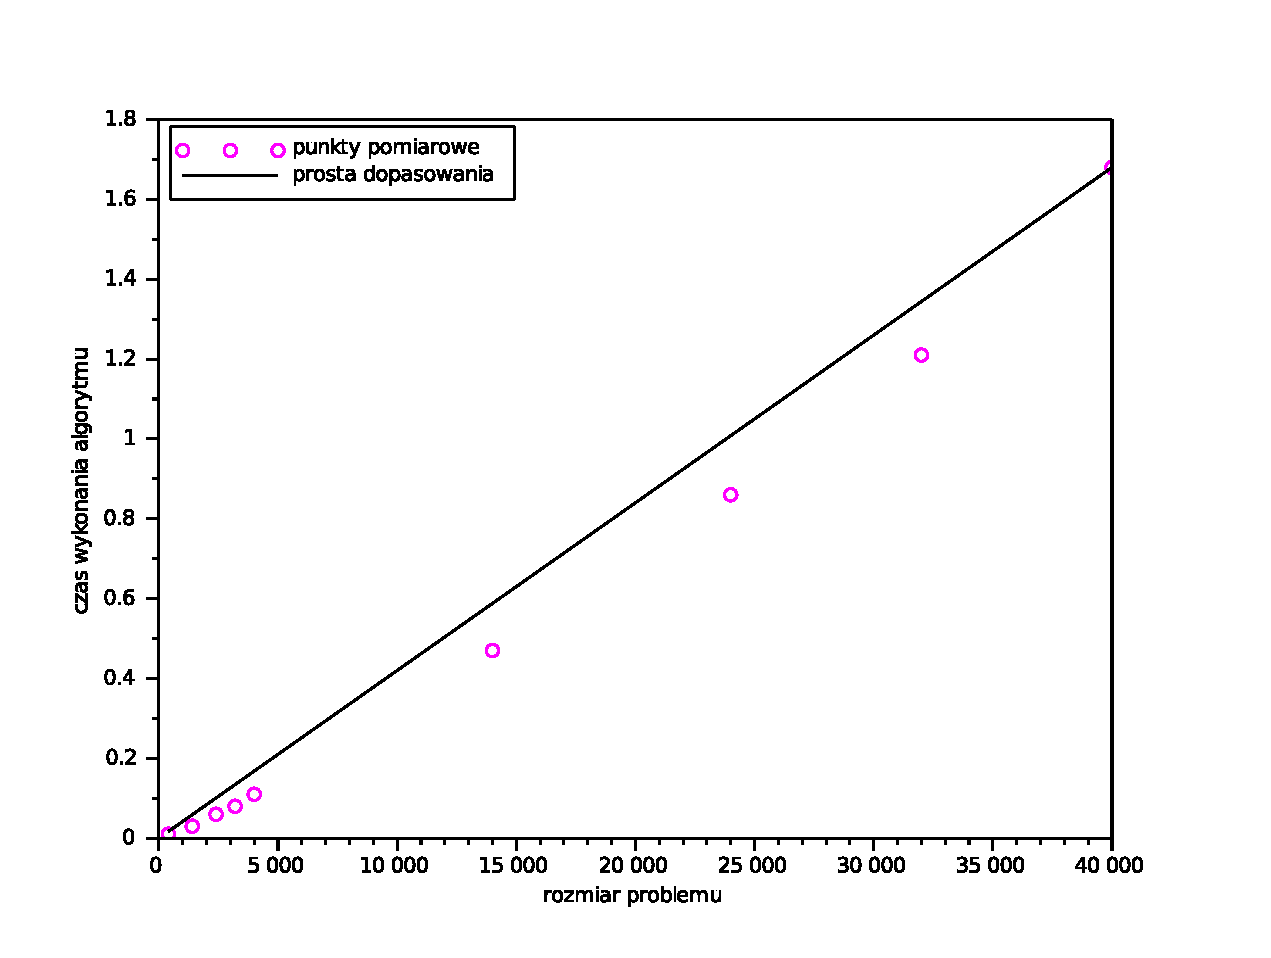
\includegraphics[width=0.95\textwidth]{dfs.pdf}
\caption{Zależność czasu wykonywania algorytmu od rozmiaru problemu dla przeszukiwania w głąb. \label{fdfs}} 
\end{figure}

\subsection{Przeszukiwanie wszerz}
Przeszukiwanie wszerz różni się od przeszukiwania w głąb użytą strukturą danych. W przypadku przeszukiwania wszerz możemy skorzystać np.: z kolejki (tak jak zostało zaimplementowane w programie). Przeszukiwane są wszystkie wierzchołki grafu sąsiadujące z wierzchołkiem początkowym, następnie sprawdzane są kolejne, aż do natrafienia na ostatni wierzchołek. Należy uważać, by nie wracać do wierzchołków wcześniej odwiedzonych (każdy można odwiedzić tylko raz). Jeżeli po przeszukaniu wszystkich wierzchołków nie znajdziemy stanu końcowego oznacza to, że nie istnieje droga między szukanymi wierzchołkami.

Przeszukiwanie wszerz ma złożoność obliczeniową w przybliżeniu liniową, co widać na rysunku \ref{fbfs}.

\begin{figure}[!htp]
\centering
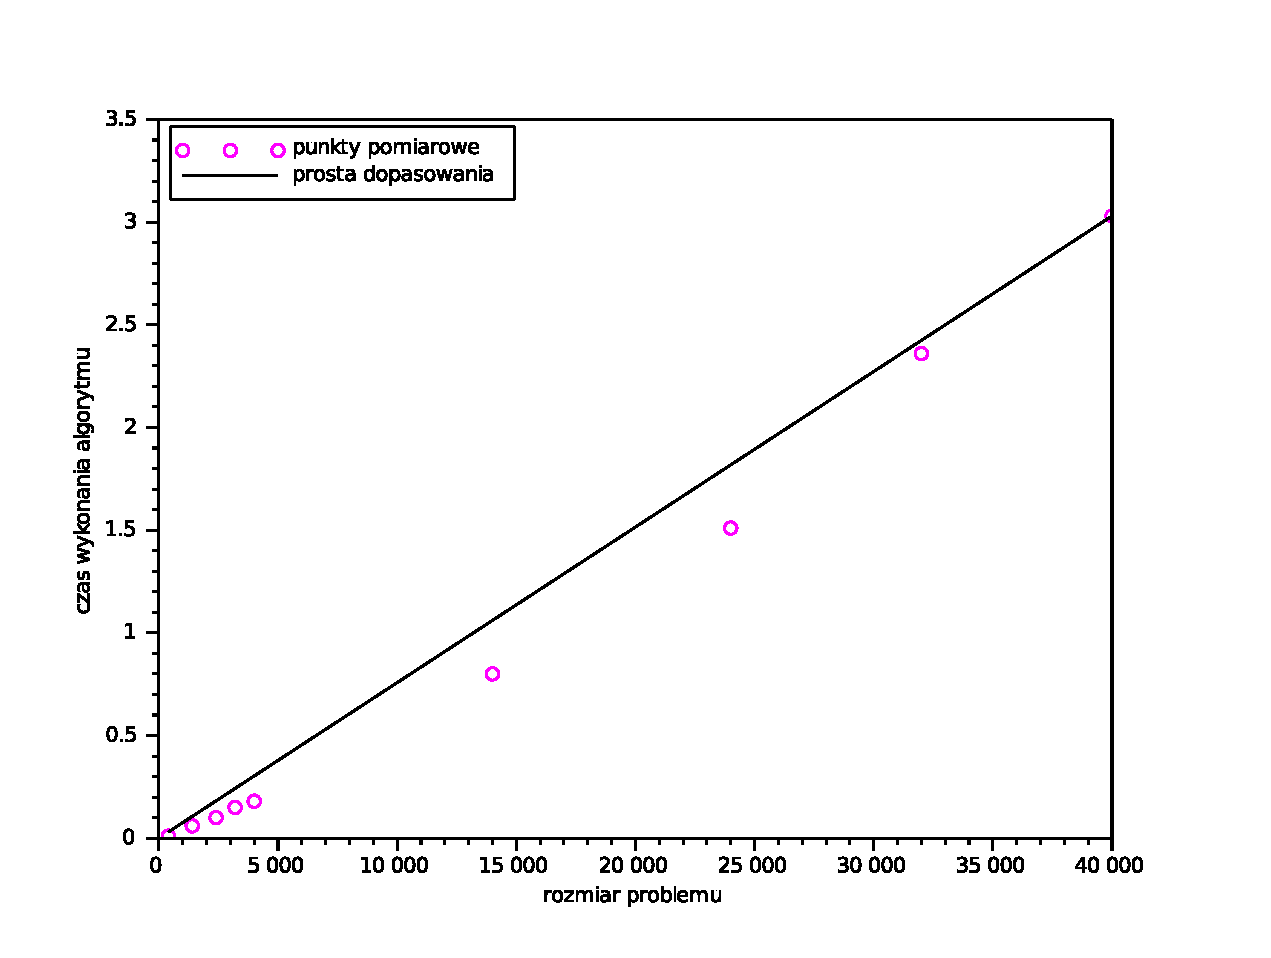
\includegraphics[width=0.95\textwidth]{bfs.pdf}
\caption{Zależność czasu wykonywania algorytmu od rozmiaru problemu dla przeszukiwania wszerz. \label{fbfs}} 
\end{figure}

\section{Podsumowanie i wnioski}
\begin{itemize}
\item Algorytmy przeszukiwania w głąb i wszerz są najczęściej stosowanymi algorytmami przeszukiwania.
\item Udało się osiągnąć rezultat zgodny z oczekiwaniami, w przypadku obu implementacji zależność jest w przybliżeniu liniowa. W najgorszym przypadku przeszukiwania mają złożoność czasową O(|V|+|E|), gdzie V to liczba węzłów, E krawędzi w grafie.
\item W przypadku zastosowanych implementacji przeszukiwanie grafu wszerz zajmuje znacznie więcej czasu.

\end{itemize}




\end{document}